\documentclass{standalone}
\usepackage{tikz}
\usepackage{ctex,siunitx}
\setCJKmainfont{Noto Serif CJK SC}
\usepackage{tkz-euclide}
\usepackage{amsmath}
\usetikzlibrary{patterns, calc,3d}
\usetikzlibrary {decorations.pathmorphing,decorations.pathreplacing,decorations.shapes}
\begin{document}
\small
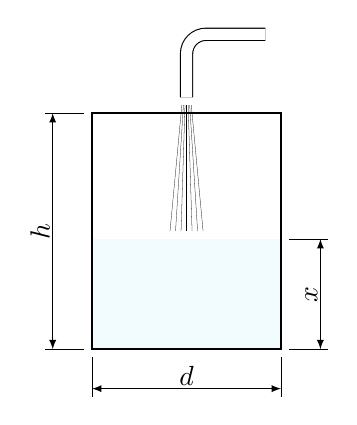
\begin{tikzpicture}[>=latex,scale=1.0,inner sep=1pt]
  \fill[cyan!10!white,opacity=0.5](-1.2,0)rectangle(1.2,1.4);
  \draw[semithick](-1.2,0)rectangle(1.2,3.0);
  \draw[very thin](-1.2,-0.1)--(-1.2,-0.6)(1.2,-0.1)--(1.2,-0.6)(-1.3,0)--(-1.8,0)(-1.3,3)--(-1.8,3)(1.3,0)--(1.8,0)(1.3,1.4)--(1.8,1.4);
  \draw[very thin,<->](-1.2,-0.5)--(1.2,-0.5)node[midway,above]{$d$};
  \draw[very thin,<->](-1.7,0)--(-1.7,3)node[midway,sloped,above]{$h$};
  \draw[very thin,<->](1.7,0)--(1.7,1.4)node[midway,sloped,above]{$x$};
  \draw[double,double distance=4pt,rounded corners=7pt](0,3.2)--(0,4)--(1,4);
  \foreach \x in {0,1,2,3}
  {
    \draw[ultra thin](0.02*\x,3.1)--(0.07*\x,1.5);
    \draw[ultra thin](-0.02*\x,3.1)--(-0.07*\x,1.5);
  }
\end{tikzpicture}
\end{document}